\begin{figure}[t]
\centering
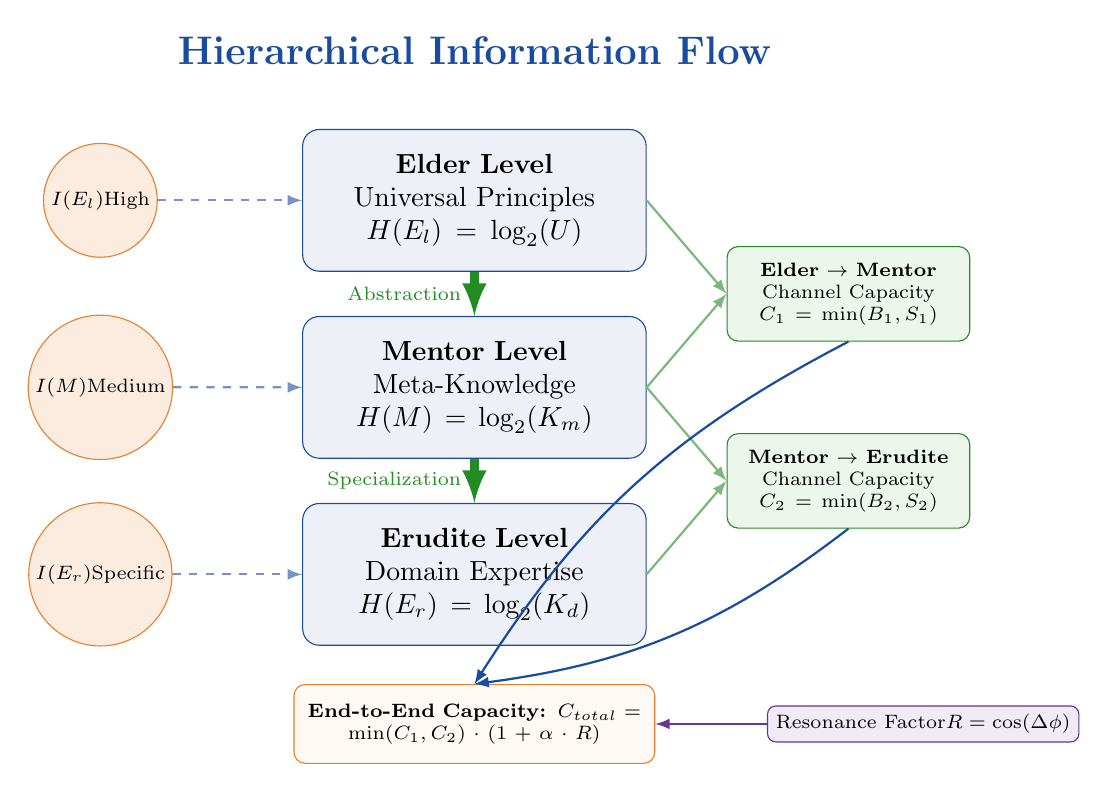
\begin{tikzpicture}[scale=0.95]
    % Define Elder color palette
    \definecolor{elderblue}{RGB}{25,76,158}
    \definecolor{elderorange}{RGB}{231,127,43}
    \definecolor{eldergreen}{RGB}{34,139,34}
    \definecolor{elderpurple}{RGB}{102,51,153}
    
    % Define clean, modern styles
    \tikzset{
        level/.style={
            draw=elderblue,
            fill=elderblue!8,
            rounded corners=6pt,
            minimum width=4cm,
            minimum height=1.8cm,
            text width=3.8cm,
            align=center,
            font=\normalsize,
            inner sep=8pt
        },
        flow/.style={
            draw=eldergreen,
            fill=eldergreen!8,
            rounded corners=4pt,
            minimum width=3cm,
            minimum height=1.2cm,
            text width=2.8cm,
            align=center,
            font=\scriptsize,
            inner sep=4pt
        },
        equation/.style={
            draw=elderorange,
            fill=elderorange!5,
            rounded corners=4pt,
            minimum width=4.5cm,
            minimum height=1cm,
            text width=4.3cm,
            align=center,
            font=\scriptsize,
            inner sep=4pt
        },
        arrow/.style={
            ->,
            elderblue,
            thick,
            >=latex
        },
        info/.style={
            draw=elderorange,
            fill=elderorange!15,
            circle,
            minimum size=1.4cm,
            font=\scriptsize,
            inner sep=2pt
        }
    }
    
    % Title
    \node[font=\Large\bfseries, elderblue] at (0, 7.5) {Hierarchical Information Flow};
    
    % Central hierarchy column
    \node[level] (elder) at (0, 5.5) {\textbf{Elder Level}\\Universal Principles\\$H(E_l) = \log_2(U)$};
    \node[level] (mentor) at (0, 3) {\textbf{Mentor Level}\\Meta-Knowledge\\$H(M) = \log_2(K_m)$};
    \node[level] (erudite) at (0, 0.5) {\textbf{Erudite Level}\\Domain Expertise\\$H(E_r) = \log_2(K_d)$};
    
    % Information content indicators (left side)
    \node[info] (i_elder) at (-5, 5.5) {$I(E_l)$\\High};
    \node[info] (i_mentor) at (-5, 3) {$I(M)$\\Medium};
    \node[info] (i_erudite) at (-5, 0.5) {$I(E_r)$\\Specific};
    
    % Flow channels (right side)
    \node[flow] (flow1) at (5, 4.25) {\textbf{Elder $\to$ Mentor}\\Channel Capacity\\$C_1 = \min(B_1, S_1)$};
    \node[flow] (flow2) at (5, 1.75) {\textbf{Mentor $\to$ Erudite}\\Channel Capacity\\$C_2 = \min(B_2, S_2)$};
    
    % Main information flow arrows
    \draw[arrow, line width=3pt, eldergreen] (elder) -- (mentor) node[midway, left, font=\scriptsize] {Abstraction};
    \draw[arrow, line width=3pt, eldergreen] (mentor) -- (erudite) node[midway, left, font=\scriptsize] {Specialization};
    
    % Information content connections
    \draw[arrow, elderblue!60, dashed] (i_elder) -- (elder);
    \draw[arrow, elderblue!60, dashed] (i_mentor) -- (mentor);
    \draw[arrow, elderblue!60, dashed] (i_erudite) -- (erudite);
    
    % Flow monitoring connections
    \draw[arrow, eldergreen!60] (elder.east) -- (flow1.west);
    \draw[arrow, eldergreen!60] (mentor.east) -- (flow1.west);
    \draw[arrow, eldergreen!60] (mentor.east) -- (flow2.west);
    \draw[arrow, eldergreen!60] (erudite.east) -- (flow2.west);
    
    % System capacity equation at bottom
    \node[equation] (capacity) at (0, -1.5) {
        \textbf{End-to-End Capacity:} $C_{total} = \min(C_1, C_2) \cdot (1 + \alpha \cdot R)$
    };
    
    % Resonance enhancement indicator
    \node[draw=elderpurple, fill=elderpurple!10, rounded corners=3pt, font=\scriptsize, inner sep=3pt] (resonance) at (6, -1.5) {
        Resonance Factor\\$R = \cos(\Delta\phi)$
    };
    
    % Connect capacity elements
    \draw[arrow, elderblue] (flow1.south) to[bend right=15] (capacity.north);
    \draw[arrow, elderblue] (flow2.south) to[bend left=15] (capacity.north);
    \draw[arrow, elderpurple] (resonance) -- (capacity);
    
\end{tikzpicture}
\caption{Information flow and capacity in the Elder system's hierarchical structure. Information content at each level (Elder, Mentor, Erudite) is represented by the Shannon mutual information between entity states and parameters. Information flows between hierarchical levels through channels with specific capacities determined by signal-to-noise ratios and dimensionality. The end-to-end capacity from Elder to Erudite is bounded by the minimum capacity of the individual channels, identifying potential bottlenecks. Resonance mechanisms enhance channel capacity by improving signal quality. The system exhibits synergistic information that scales superlinearly with the number of entities, contributing to the total information content beyond the sum of individual entity information.}
\label{fig:hierarchical_information}
\end{figure}